\documentclass[11pt]{article}
\usepackage[italian]{babel}
\usepackage[utf8]{inputenc}	% Para caracteres en español
\usepackage{amsmath,amsthm,amsfonts,amssymb,amscd}
\usepackage{multirow,booktabs}
\usepackage[table]{xcolor}
\usepackage{fullpage}
\usepackage{lastpage}
\usepackage{enumitem}
\usepackage{fancyhdr}
\usepackage{mathrsfs}
\usepackage{wrapfig}
\usepackage{graphicx}
\graphicspath{ {./images/} }
\usepackage{setspace}
\usepackage{calc}
\usepackage{multicol}
\usepackage{cancel}
\usepackage[retainorgcmds]{IEEEtrantools}
\usepackage[margin=3cm]{geometry}
\usepackage{amsmath}
\newlength{\tabcont}
\setlength{\parindent}{0.0in}
\setlength{\parskip}{0.05in}
\usepackage{empheq}
\usepackage{framed}
\usepackage[most]{tcolorbox}
\usepackage{xcolor}
\usepackage{FiraSans}
\usepackage[numbered,framed]{matlab-prettifier}

\let\ph\mlplaceholder % shorter macro
\lstMakeShortInline"

\lstset{
  style              = Matlab-editor,
  basicstyle         = \mlttfamily,
  escapechar         = ",
  mlshowsectionrules = true,
}

\colorlet{shadecolor}{orange!15}
\parindent 0in
\parskip 12pt
\geometry{margin=1in, headsep=0.25in}
\theoremstyle{definition}
\newtheorem{defn}{Definizione}
\newtheorem{reg}{Regola}
\newtheorem{oss}{Osservazione}
\newtheorem{exer}{Esecizio}
\newtheorem{dimo}{Dimostrazione}
\newtheorem{note}{Nota}
\newtheorem{thm}{Teorema}[section] % reset theorem numbering for each chapter

\theoremstyle{plain}
\newcommand{\restr}[2]{%
\mathchoice{%
\restriction{#1}{#2}{\displaystyle}%
}{%
\restriction{#1}{#2}{\textstyle}%
}{%
\restriction{#1}{#2}{\scriptstyle}%
}{%
\restriction{#1}{#2}{\scriptscriptstyle}%
}%
}

\newlength{\totbarheight}
\newlength{\bardepth}




\begin{document}

\title{Interpolazione Polinomiale}
\author{Guglielmo Bartelloni}
\maketitle

\thispagestyle{empty}

\begin{center}
{\LARGE \bf 31 Marzo 2022}\\
\end{center}

\section{Formule di quadratura}

Il problema, in questo caso, è quello di ottenere una approssimazione di un integrale definito:
\[
	I(f)=\int_{a}^{b}f(x)dx\ \ \ \ (1)
.\] 

Assumiamo che $f\in C[a,b]$ (cioè che la funzione sia continua nell'intervallo), ed anche che $a<b$ , perchè altrimenti basterebbe cambiare di segno all'integrale, ed anche che $-\infty<a<b<+\infty$, ovvero non si tratta di un integrale improprio.

Se conoscessimo una primitiva di $f(x)$ chiamiamola $F(x)$ allora:
\[
	\int_{a}^{b}f(x)dx=F(b)-F(a)
.\] 

Tuttavia, la primitiva di una funzione \textbf{non si sa calcolare sempre}, per cui vogliamo definire dei metodi numerici di approssimazione per (1).

Vogliamo prima studiare il condizionamento del problema (controlliamo se il risultato cambia al perturbare dei dati in ingresso). In questo caso, quindi, vogliamo vedere quanto vale la differenza $|I(f)-I(\overline{f})|$ essendo $\overline{f(x)}$ una perturbazione della funzione integranda, con le stesse proprieta ($\overline{f}\in C[a,b]$. Si ottiene che:
\[
	|I(f)-I(\overline{f})|=|\int_{a}^{b}f(x)dx-\int_{a}^{b}\overline{f(x)}dx|=
.\] 
\[
=|\int_{a}^{b}(f(x)-\overline{f(x)})dx\le \int_{a}^{b}|f(x)-\overline{f(x)}|dx\le ||f-\overline{f}||\int_{a}^{b}dx=(b-a)||f-\overline{f}||
.\] 

In questo caso
\[
	||f-\overline{f}||=max_{a\le x\le b}|f(x)-\overline{f(x)}|
.\] 

Riassumendo, abbiamo ottenuto che:
\[
	|I(f)-I(\overline{f})|\le (b-a)||f-\overline{f}||
.\] 

La norma è una misura dell'errore su i dati in ingresso, il primo mebro invece, è la misura dell'errore sul risultato. (l'ampiezza dell'intervallo è il numero di condizionamento del problema).

Pertanto, ad esempio:
\[
	\int_{0}^{10^{25}}sin(x)dx \to k=10^{25}\to problema\ malcondizionato
.\] 

Viceversa:
\[
	\int_{0}^{1}e^{sin\sqrt{1+tan(1+x)} }dx \to k=1\to problema\ bencondizionato
.\] 

Quindi il tutto dipende dall'ampiezza dell'intervallo.

Avendo definito il numero di condizionamento del problema (1), occupiamoci della sua approssimazione mediante una opportuna \textbf{formula di quadratura}.
Quest'ultima è definita dall'integrale di una conveniente approssimazione $\phi(x) \approx f(x)$, $x\in[a,b]$, di cui si sappia calcolare facilmente l'integrale esatto:
\[
	I(f)\approx I(\phi)
.\] 

Rimane, quindi, da specializzare l'approssimazione $\phi$ . A riguardo, ci ricoiamo che l'integrale di un polinomio si sa calcolare facilmente, per cui sceglieremo $\phi \in \Pi$. In particolare, utilizzeremo, come approssimazione di f(x), il suo polinomio interpolante su $n+1$ ascisse equidistanti:
\[
x_{i}=a+ih\ \ \ i=0,...,n\ \ \ h=\frac{b-a}{n}
.\] 

Come al solito, denoteremo con $f_{i}\equiv f(x_{i})$ , $i=0,...,n$, il valore assunto dalla funzione integranda in tali ascisse.

Per le finalità che ci proponiamo, sarà conveniente scegliere la \textbf{forma di Lagrange} del polinomio interpolante:
\[
	p(x)=\sum_{i=0}^{n} f_{i}L_{in}(x)
.\] 

essendo $L_{in}(x)=\prod_{j=0\\ j = i}^{n} \frac{x-x_{j}}{x_{i}-x_{j}}$ per $i=0,...,n$ è l'i-esimo polinomio di base di Lagrange

Andiamo, quindi, a calcolare:
\[
	I(p)\equiv I_n(f)
.\] 

che definira la \textbf{formula di quadratura di Newton-Cotes di grado n}

Si ottiene:
\[
	I(p)=\int_{a}^{b}\sum_{i=0}^{n} f_{i}L_{in}(x)dx=\sum_{i=0}^{n} f_{i}\int_{a}^{b}L_{in}(x)dx
.\] 

analizziamo uno dei generici pesi della quadratura:
\[
	\int_{a}^{b}L_{in}(x)dx=\int_{a}^{b}\prod_{j=0\\ j = i}^{n} \frac{x-x_{j}}{x_{i}-x_{j}}dx=(*)
.\] 

Per renderlo indipendente dall'intervallo $[a,b]$, definiamo la trasformazione
\[
x=a+th \ \ \ \ h=\frac{b-a}{n}
.\] 

otteniamo che:
\begin{enumerate}
	\item $t\in [0,n]$ 
	\item $dx=hdt$ 
	\item $x_{i}=a+ih$ 
\end{enumerate}

pertanto:
\[
	(*)=h\int_{0}^{n}\prod_{j=0 j=i}^{n} \frac{a+th-a-jh}{a+ih-a-jh}dt=h\int_{0}^{n}\prod_{j=0 j=i}^{n} \frac{t-j}{i-j}dt=
\] 

l'espressione sopra dipende non piu da a e b ma da i e da n:
\[
=hc_{in}
.\] 

dove $c_{in}=\int_{0}^{n}\sum_{j=0 j\neq i}^{n} \frac{t-j}{i-j}dt$, è un coefficiente che dipende solo da i e n.

Pertanto la formula di Newton-Cotes di grado n sarà data da:
\[
	I_{n}(f)=h\sum_{i=0}^{n} c_{in}f_{i}=\frac{b-a}{n}\sum_{i=0}^{n} c_{in}f_{i}
.\] 

\begin{oss}
	I coefficienti $c_{in}$ sono dei numeri razionali.
\end{oss}

\begin{thm}
	Vale la seguente proprieta:
	\[
	\frac{1}{n}\sum_{i=0}^{n} c_{in}=1
	.\] 
\end{thm}

\begin{dimo}
	Se consideriamo $f(x)\equiv 1 \implies p(x)=f(x),\forall n\ge 1$  e, pertanto, $I(1)\equiv I_{n}(1),\forall n\ge 1$. Ovvero:
	\[
	\int_{a}^{b}1dx=\frac{b-a}{n}\sum_{i=0}^{n} 1c_{in} \implies 1=\frac{1}{n}\sum_{i=0}^{n} c_{in}
	.\] 

come volevamo dimostrare
\end{dimo}

\subsection{Condizionamento della formula}

Prima di procedere oltre, andiamo a studiare il condizionamento della generica formula di Newton-Cotes, ovvero vedere come la differenza $|I_n(f)-I_n(\overline{f})|$ dipende dal $||f-\overline{f}||$ (analogamente a quanto visto nel caso di $I(f)$ ).

Sviluppando i conti, si ottiene:
\[
	|I_n(f)-I_n(\overline{f})|= |\frac{b-a}{n}\sum_{i=0}^{n} f_ic_{in}-\frac{b-a}{n}\sum_{i=0}^{n} \overline{f}_{i}c_{in}|=\frac{b-a}{n}|\sum_{i=0}^{n} (f_i-\overline{f}_{i})c_{in}|\le \frac{b-a}{n}|\sum_{i=0}^{n} |f_i-\overline{f}_{i}|c_{in}|
.\] 

\[
	\frac{b-a}{n}||f_i-\overline{f}_{i}||\sum_{i=0}^{n} |c_{in}|= (b-a)[\frac{1}{n}\sum_{i=0}^{n} |c_{in}|]||f-\overline{f}||
.\] 

In conclusione:
\[
	|I_n(f)-I_n(\overline{f})|\le (b-a)[\frac{1}{n}\sum_{i=0}^{n} |c_{in}|]||f-\overline{f}||
.\] 

Primo membro è l'errore sul risultato, la norma è l'errore in ingresso, il resto del secondo membro è il numero di condizionamento

\begin{oss}
	\begin{enumerate}
		\item se $c_{in}\ge 0$, $i=0,...,n$ allora $\frac{1}{n}\sum_{i=0}^{n} |c_{in}|=\frac{1}{n}\sum_{i=0}^{n} c_{in}=1$ 
		\item se vi sono coefficienti negativi, allora $\frac{1}{n}\sum_{i=0}^{n} |c_{in}|\le \frac{1}{n}\sum_{i=0}^{n} c_{in}=1$
	\end{enumerate}

	Nel caso 1) abbiamo che $k=k_n$ .

	Nel caso 2) abbiamo che $k_n>k$ 

	Il caso 1) vale per $n=1,...,7,9$ 

	Per $n>9$ il rapporto $\frac{k_n}{k}=\frac{1}{n}\sum_{i=0}^{n}|c_{in}| $ cresce molto rapidamente.
\end{oss}

Pertanto le formule di Newton-Cotes con $n>9$ non sono da utilizzare nella pratica computazionale (anche n=8 è da evitare).


\begin{center}
{\LARGE \bf 06 Aprile 2022}\\
\end{center}

Facciamo degli esempi di formule di Newton-Cotes.

Nel derivare i coefficienti di queste formule, terremo conto delle proprietà di simmetria:
\[
	c_{in}=c_{n-in},\ \ \ i=0,...,n\ \ \ (c_1)
.\] 

e del fatto che:
\[
	\sum_{i=0}^{n} c_{in}=n\ \ \ (c_2)
.\] 

Ricordiamo che:
\[
	c_{in}=\int_{0}^{n}\sum_{j=0 j\neq i}^{n} \frac{t-j}{i-j}dt\ \ \ \ i=0,...,n\ \ \ (c_3)
.\] 

Per \textbf{n=1} abbiamo solo 2 coefficienti, $c_{01}$ e $c_{11}$ Poiche dalla $c_1$  segue che $c_{01}=c_{11}$ allora si perviene a:
\[
c_{01}=c_{11}=\frac{1}{2}
.\] 

Quindi, $x_0=a$, $x_1=b$, $h=b-a$, da cui:
\[
	I_1(f)=(b-a)\frac{f(a)+f(b)}{2}
.\] 

Vediamo geometricamente cosa significa (appunti):

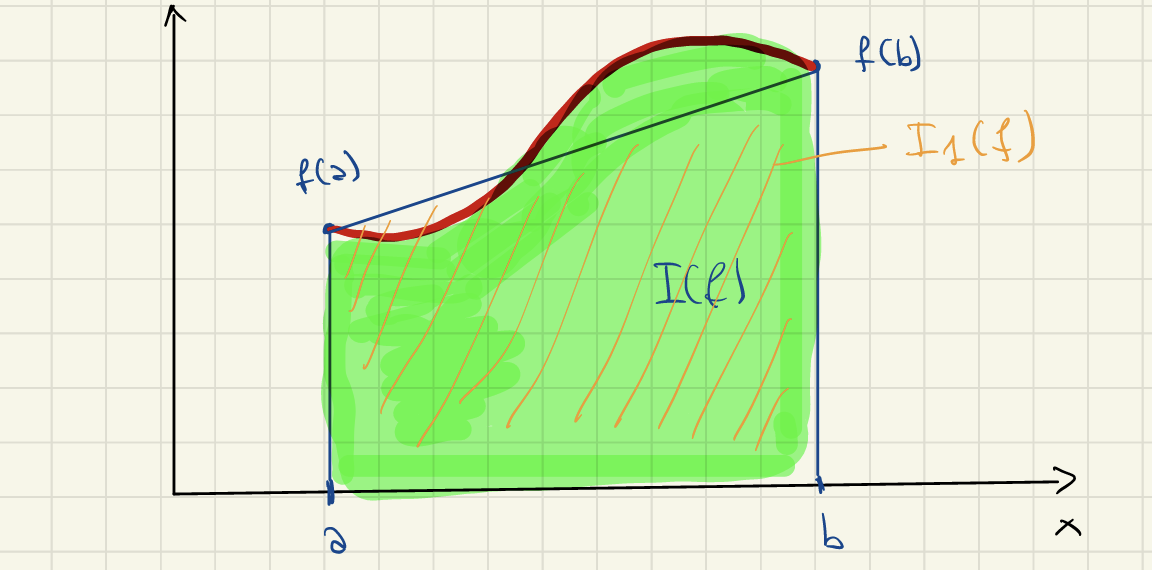
\includegraphics[width=\textwidth]{formula_trapezio}

In questo caso quindi stiamo approssimando l'integrale della funzione attraverso un trapezio rettangolo, la formula sopra infatti rappresenta proprio il calcolo dell'area di un trapezio (semisomma della basi * altezza). Si parla infatti di \textbf{metodo del trapezio}

Per \textbf{n=2} Rammendiamo che, dalle $c_1$ e $c_2$ segue che:
\[
c_{02}=c_{22}
.\] 
e
\[
c_{02}+c_{12}+c_{22}=2 \implies c_{12}=2-2c_{22}
.\] 

Pertanto ci basta calcolare $c_{22}$ per ottenere gli altri coefficienti:
\[
	c_{22}=\int_{0}^{2}\prod_{j=0 j\neq 2}^{2} \frac{t-j}{2-j}dt=\int_{0}^{2}\prod_{j=0 j\neq 2}^{2} \frac{t(t-1)}{2*1}dt=\frac{1}{2}\int_{0}^{2}\prod_{j=0 j\neq 2}^{2} (t^{2}-t)dt=
	\] 
\[
=\frac{1}{2}\int_{0}^{2}\prod_{j=0 j\neq 2}^{2} (\frac{t^{3}}{3}-\frac{t^{2}}{2})dt=\frac{1}{2}\frac{t^{2}}{6}(2t-3)_{\mkern 1mu \vrule height 2ex\mkern2mu [t=0,t=2]}=\frac{1}{3}
.\] 

Pertanto, $c_{02}=c_{22}=\frac{1}{3}$  e $c_{12}=\frac{4}{3}$ . La formula risultante sara, dunque, considerato che le asciesse sono
\[
x_0=a,x_1=\frac{a+b}{2},x_2=b,con\ \ \ h=\frac{b-a}{2}
.\] 
\[
	I_2(f)=\frac{b-a}{2}(\frac{f(a)}{3}+\frac{4}{3}f(\frac{a+b}{2})+\frac{f(b)}{3})
.\] 

	Questo definisce la \textbf{formula di simpson}.
\subsection{Calcolo dei coefficienti}
\[
c_{in}=\int_{0}^{n}\sum_{j=0 j\neq i}^{n} \frac{t-j}{i-j}dt
.\] 

$c_{in}$ sarà necessariamente un numero razionale. Vediamo di calcolarne numeratore e denominatore in modo efficiente.

\subsubsection{Denominatore}
Abbiamo formalmente che:

\[
	\sum_{j=0 j\neq i}^{n} i-j
.\] 

Questo si puo rendere in Matlab coe segue:

\lstinputlisting{codice/quadraturaDenominatore.m}

\subsubsection{Numeratore}
Pertanto rimane da calcolare
\[
num=\int_{0}^{n}\sum_{j=0 j\neq i}^{n} t-j dt
.\] 
che è l'integrale di un polinomio monico, le cui radici sono gli interi da 0 a n, escluso i. Possiamo calcolare i coefficineti di questo polinomio ( che sono degli interi) mediante la function \textbf{poly} di Matlab:

\lstinputlisting{codice/quadraturaNumeratore.m}

considerato che
\[
	a=[a_n, a_{n-1}, ..., a_0]
.\] 

con $a_j$ il coefficiente $x_{j}$, otteniamo che l'integrale del polinomio, sarà un polinomio con coefficienti:
\[
	[\frac{a_n}{n+1},\frac{a_{n-1}}{n}, .... , \frac{a_0}{1}, 0]
.\] 
Ne calcoliamo i coefficinenti, sovrascrivendo il vettore a come segue:

\lstinputlisting{codice/vettoreA.m}

Per calcolare num, sarà sufficiente valutare il polinomio cosi ottenuto in n:
per far questo possiamo utilizzare la function polyval di Matlab:
\lstinputlisting{codice/num.m}

Pertanto $c_{in}=\frac{num}{dem}$.

Se utilizzate il formato \textbf{format rational} (che ci da il numero di frazione). Questa function risulta essere esatta per le formule di Newton-Cotes di interesse ($n\le 9$). Mettendo i pezzi insieme si è in grado di costruire una function che calcola i coefficienti in forma razionale.

\section{Errore di quadratura}
Definiamo:
\[
	E_{n}(f)=I(f)-I_{n}(f)= \int_{a}^{b}f(x)dx-\int_{a}^{b}p_n(x)dx=\int_{a}^{b}e_n(x)dx
.\] 

Dove $e_n(x)$ è l'errore di interpolazione, abbiamo visto che:
\[
	e_n(x)=f[x_0,...,x_n,x]w_{n+1}(x)
.\] 

con $w_{n+1}=\prod_{i=0}^{n} (x-x_{i})$. Pertanto:
\[
	E_n(f)=\int_{a}^{b}e_n(x)dx=\int_{a}^{b}f[x_0,...,x_n,x]w_{n+1}(x)dx
.\] 

A riguardo si puo dimostrare il seguente risultato:
\begin{thm}
	Se $f\in C^{n+k}[a,b]$, con
		  \begin{equation}
		    k=
		    \begin{cases}
		      1, & \text{se}\ n dispari \\
		      2, & \text{se}\ n pari
		    \end{cases}
		  \end{equation}
	
		  allora $\forall V_n$ costante dipendnete solo da n e $\epsilon \in [a,b]$:
		  \[
			  E_n(f)=V_nf^{n+k}(\epsilon)(\frac{b-a}{n})^{n+k+1}=(*)
		  .\] 
	
\end{thm}

\begin{oss}
	Pertanto, la formula di Newton-Cotes di grado n è esatta per polinomi di grado 
	  \begin{equation}
	    \begin{cases}
	      n, & \text{se}\ n dispari \\
	      n+1, & \text{se}\ n pari
	    \end{cases}
	  \end{equation}
	
\end{oss}

Se esaminiamo (*) notiamo che, se la funzione è molto regolare, allora: 
\[
	\frac{(b-a)}{n}^{n+k+1}\to 0,n\to \infty
.\] 

Quindi, questo ci spingerebbe ad utilizzare formule di Newton-Cotes di grado elevato.

D'altronde, per $n\ge 10$, sappiamo che $\frac{k_n}{k}\to \infty$, $n\to \infty$, anche questo esponenzialennte. Quindi doremo escogitare delle modiciche algoritmiche che consentono di ridurre l'errore senza aumentare il grado della formulta.

\begin{center}
{\LARGE \bf 07 Aprile 2022}\\
\end{center}

\section{Formule composite di Newton-Cotes}

In questo caso l'idea è suddividere l'intervallo di integrazione in più sottointervalli (utilizzando sempre delle ascisse equidistanti), ed applicare in ciascuno di questi una formula di Newton-Cotes di grado k fissato.

\subsection{Caso del trapezio}

Esaminiamo la formula composita nel caso del trapezio:
\[
	I(f)=\frac{(b-a)}{2}(f(a)+f(b))
.\] 

Supponendo di avere le n+1 ascisse equidistanti $x_{i}=a+ih$, $i=0,...,n,h=(\frac{b-a}{n})$ 

GRAFICO Appunti

Formalmente (faccio la somma dei mini intervalli):
\[
	I(f)=\int_{a}^{b}f(x)dx=\sum_{i=1}^{n} \int_{x_{i-1}}^{x_{i}}f(x)dx\approx \sum_{i=1}^{n} \frac{x_{i}-x_{i-1}}{a}(f_i-f_{i-1})=\frac{b-a}{n}\sum_{i=1}^{n} \frac{1}{2}(f_{i}+f_{i-1})=
\] 

\[
	=\frac{b-a}{n}(\frac{f(a)}{2}+\sum_{i=1}^{n-1} f_{i}+\frac{f(b)}{2})\equiv I_1^{n}(f)
.\] 

Che è la \textbf{formula composita dei trapezi}.

\subsubsection{Errore della formula composita dei trapezi}

Analizziamo l'errore di qudratura che si ha in questo caso:
\[
	E_1^{n}(f)=I(f)-I_1^{n}(f)=\sum_{i=1}^{n}[ \int_{x_{i-1}}^{x_{i}}f(x)dx-\frac{x_{i}-x_{i-1}}{2}(f_{i}+f_{i-1})]=
\] 
\[
	=\sum_{i=1}^{n} V_1f^{2}(\epsilon_i)(\frac{b-a}{n})^{3}=V_1(\frac{b-a}{n})^{3}\sum_{i=1}^{n} f^{2}(\epsilon_i)=V_1nf^{2}(\epsilon)(\frac{b-a}{n})^{3})=
\] 

Dove $\epsilon \in [a,b]$ 

\[
	=V_1(b-a)f^{2}(\epsilon)(\frac{b-a}{n})^{2}\to 0\ \ \ per\ n\to \infty
.\] 

Quindi più aumentiamo gli intervalli più si arriva ad avvicinarsi all'integrale della funzione.


\begin{oss}
	Se $f(x)$ è una funzione periodica in $[a,b]$ (tipicamente, $[a,b]=[0,2\pi]$, $f(x)=cos(jx)=sin(jx)$ $j\in N$)

	In questo caso $f(a)=f(b)$. Pertanto:
	\[
		I_1^{n}(f)=h\sum_{i=0}^{n-1} f_{i}
	.\] 
\end{oss}


\subsection{Caso della formula di Simpson}
Facciamo un ragionamento analogo per la formula di Simpson:
\[
	I_2(f)=\frac{(b-a)}{2}(\frac{f(a)}{3}+\frac{4}{3}f(\frac{a+b}{2})+\frac{f(b)}{3})
.\] 

questa è la formula di base. Se utilizziamo n+1 ascisse $x_{i}=a+ih,i=0,...,n,h=\frac{b-a}{n}$ possiamo applicare, su ciascun sottointervallo $[x_{2(i-1)},x_{2i}],i=1,...,\frac{n}{2},$ la fomrula di Simpson base:
\[
	I(f)=\int_{a}^{b}f(x)dx=\sum_{i=1}^{\frac{n}{2}} \int_{x_{2(i-1)}}^{x_{2i}}f(x)dx\approx \sum_{i=1}^{\frac{n}{2}} \frac{x_{2i}-x_{2(i-1)}}{2*3}(f_{2(i-1)}+4f_{2i-1}+f_{2i})=
\] 
\[
	=(\frac{b-a}{n})\frac{1}{3}\sum_{i=1}^{\frac{n}{2}} (f_{2(i-1)}+4f_{2i-1}+f_{2i})=
\] 

I dispari vengono moltiplicati con 4 e pari vengono moltiplicati per 2(?)
\[
	=\frac{1}{3}(\frac{b-a}{n}(4\sum_{i=1}^{\frac{n}{2}} f_{2i-1}+2\sum_{i=1}^{\frac{n}{2}-1} f_{2i}+f(a)+f(b))
.\] 

Questa definisce la \textbf{formula composita di Simpson}.

Essa è applicabile se n è multiplo di 2.
\begin{oss}
	In generale, la formula composita di Newton-Cotes di grado k su n+1 punti, è applicabile se n è multiplo di k.
\end{oss}

\subsubsection{Errore della formula composita di Simpson}
In questo caso:
\[
	E_2^{n}(f)=I(f)-I_2^{n}(f)=\sum_{i=1}^{\frac{n}{2}} [\int_{x_{2(i-1)}}^{x_{2i}}f(x)dx-\frac{x_{2i}-x_{2i-1}}{6}(f_{2(i-1)}+4f_{2i-1}+f_{2i})]=
\] 

dove $x_{2i}-x_{2i-1}=2(\frac{b-a}{n})$ 

\[
	=\sum_{i=1}^{\frac{n}{2}} V_2f^{n}(\epsilon_i)(\frac{b-a}{n})^{5}=V_2(\frac{b-a}{n})^{5}\sum_{i=1}^{\frac{n}{2}} f^{4}(\epsilon_i)=V_2(\frac{b-a}{n})^{5}\frac{h}{2}f^{4}(\epsilon)=V_2 \frac{b-a}{2}f^{4}(\epsilon)(\frac{b-a}{n})^{4}\to 0\ \ \ per\ n\to \infty
.\] 

Procedendo analogamete per una generica formula composita di grado m su n+1 punti equidistanti con n multiplo di m, si otterrà: 
\[
	E_{m}^{n}(f)=V_m\frac{(b-a)}{m}f^{m+k}(\epsilon)(\frac{b-a}{n})^{m+k}
.\] 
con
  \begin{equation}
    k=
    \begin{cases}
      1, & \text{se}\ m\ dispari \\
      2, & \text{se}\ m\ pari
    \end{cases}
  \end{equation}

con $f\in C^{m+k}[a,b],\epsilon \in [a,b]$ 

Ovviamente se $n\to \infty$ allora il tutto $\to 0$ 
\begin{oss}
	Per applicare una qualunque delle predette formule sono necessarie \textbf{n+1} valutazioni funzionali di $f(x)$, che rappresentano il costo computazionale della formula.
\end{oss}

A titolo di esempio vediamo il caso della formula composita dei trapezi in Matlab

In ingresso a,b,f,n

\lstinputlisting{codice/compositeTrapezio.m}



\end{document}



